% Document information
\newcommand{\titleinfo}{Zusammenfassung DigMe}
\newcommand{\authorinfo}{Sandro Pedrett}
\newcommand{\version}{1.0}
\newcommand{\versioninfo}{HS22}
% Header
\include{Template/Header}

% Max 8 seiten (4A seiten)

% Setup Source Code
\lstset{ 
	backgroundcolor=\color{white},   % choose the background color; you must add \usepackage{color} or \usepackage{xcolor}; should come as last argument
	basicstyle=\footnotesize,        % the size of the fonts that are used for the code
	breakatwhitespace=true,         % sets if automatic breaks should only happen at whitespace
	breaklines=true,                 % sets automatic line breaking
	captionpos=b,                    % sets the caption-position to bottom
	commentstyle=\color{ForestGreen},    % comment style
	escapeinside={\%*}{*)},          % if you want to add LaTeX within your code
	extendedchars=true,              % lets you use non-ASCII characters; for 8-bits encodings only, does not work with UTF-8
	frame=single,	                   % adds a frame around the code
	keepspaces=true,                 % keeps spaces in text, useful for keeping indentation of code (possibly needs columns=flexible)
	language=VHDL,                      % the language of the code
	numbersep=5pt,                   % how far the line-numbers are from the code
	rulecolor=\color{black},         % if not set, the frame-color may be changed on line-breaks within not-black text (e.g. comments (green here))
	showspaces=false,                % show spaces everywhere adding particular underscores; it overrides 'showstringspaces'
	showstringspaces=false,          % underline spaces within strings only
	showtabs=false,                  % show tabs within strings adding particular underscores
	stepnumber=2,                    % the step between two line-numbers. If it's 1, each line will be numbered
	tabsize=2,	                   % sets default tabsize to 2 spaces
	title=\lstname,                   % show the filename of files included with \lstinputlisting; also try caption instead of title
	stringstyle=\ttfamily\color{red!50!brown}
}

% Document
\begin{document}

\section{SoC}
Zynq-7000 Übersicht
\begin{center}
	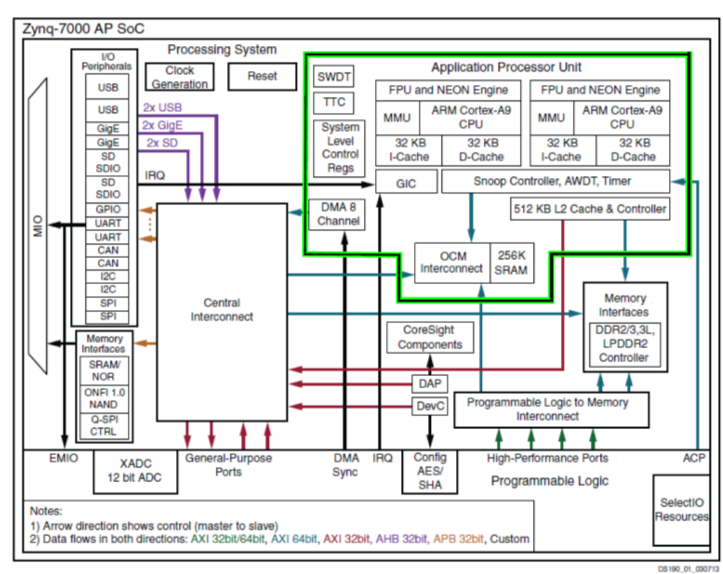
\includegraphics[width=\columnwidth]{Images/soc}
\end{center}

Ein einzelner Slice aus dem PL teil
\begin{center}
	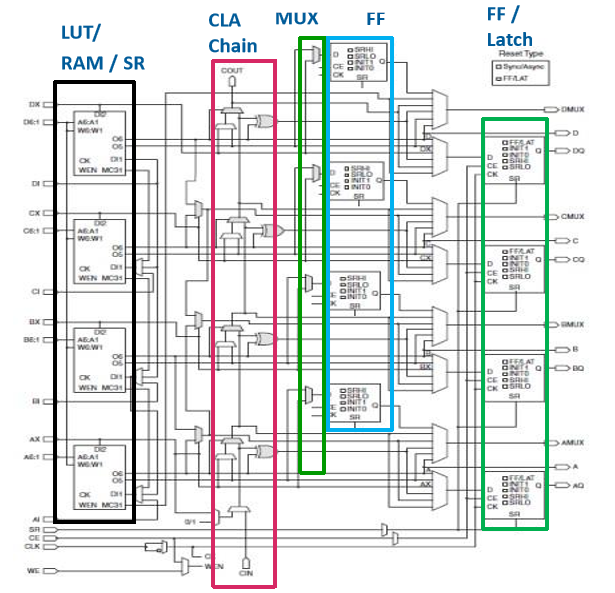
\includegraphics[width=\columnwidth]{Images/slice}
\end{center}

Ein DSP
\begin{center}
	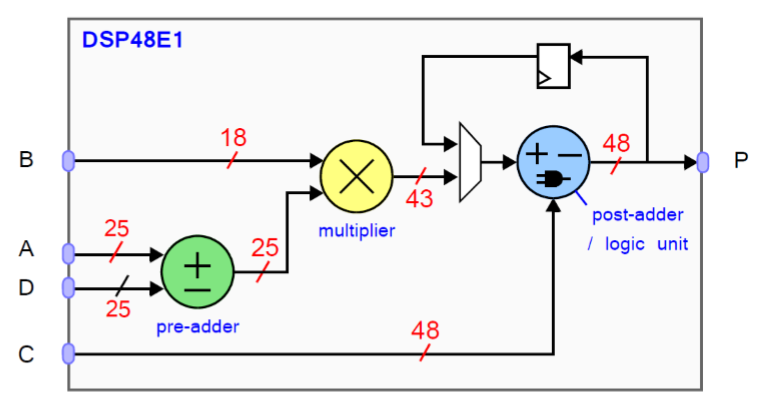
\includegraphics[width=\columnwidth]{Images/dsp}
\end{center}

\section{Constraints}
Es existieren drei verschiedene Constraints, welche sequentiell in der TCL Console verarbeitet werden.
\begin{itemize}[nosep]
	\item Physical Constraints (I/O placement)
	\item Timing Constraints (Clock definitions)
	\item Configuration Constraints (configuration, bitstream generation)
\end{itemize}

\subsection{XDC Format}
Constraints können in einem XDC File oder direkt in VHDL durch ein Attribut gesetzt werden.
\begin{lstlisting}
-- VHDL signal clk\_100MHz zu Pin Y9
set_property PACKAGE_PIN Y9 [get_ports clk_100MHz]
set_property IOSTANDARD LVCMOS33 [get_ports clk_100MHz]

-- Pull up for resetn signal
set_property PULLTYPE PULLUP [get_ports resetn]
\end{lstlisting}

Vivado IO Planner
\begin{center}
	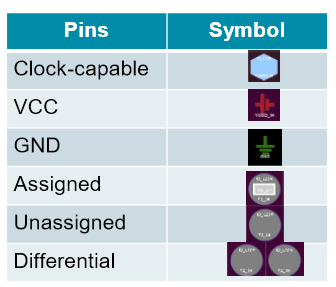
\includegraphics[width=0.4\columnwidth]{Images/ioplanner}
\end{center}

\subsection{Timing}
\begin{itemize}[nosep]
\item \textbf{Clock Distribution} delay $t_{di}$, clock latency: Zeitverzögerung gemessen vom Auftreten der Taktflanke an der Taktquelle bis zum Zustandsübergang am Ziel (Endpunkt)
\item \textbf{Clock Skew} $t_{sk}$: Ungenauigkeit der gleichen Taktflanke, die an verschiedenen Stellen im Taktbereich.
\item \textbf{Clock Jitter} $t_jt$: Variabilität der aufeinanderfolgenden Taktflanken, die an der gleichen Stelle ankommen.
\item \textbf{Slack}: Differenz zwischen benötigter Zeit und Ankunftszeit, auch als Marge bekannt. Negativer Slack => Zeitproblem
\end{itemize}
\begin{center}
	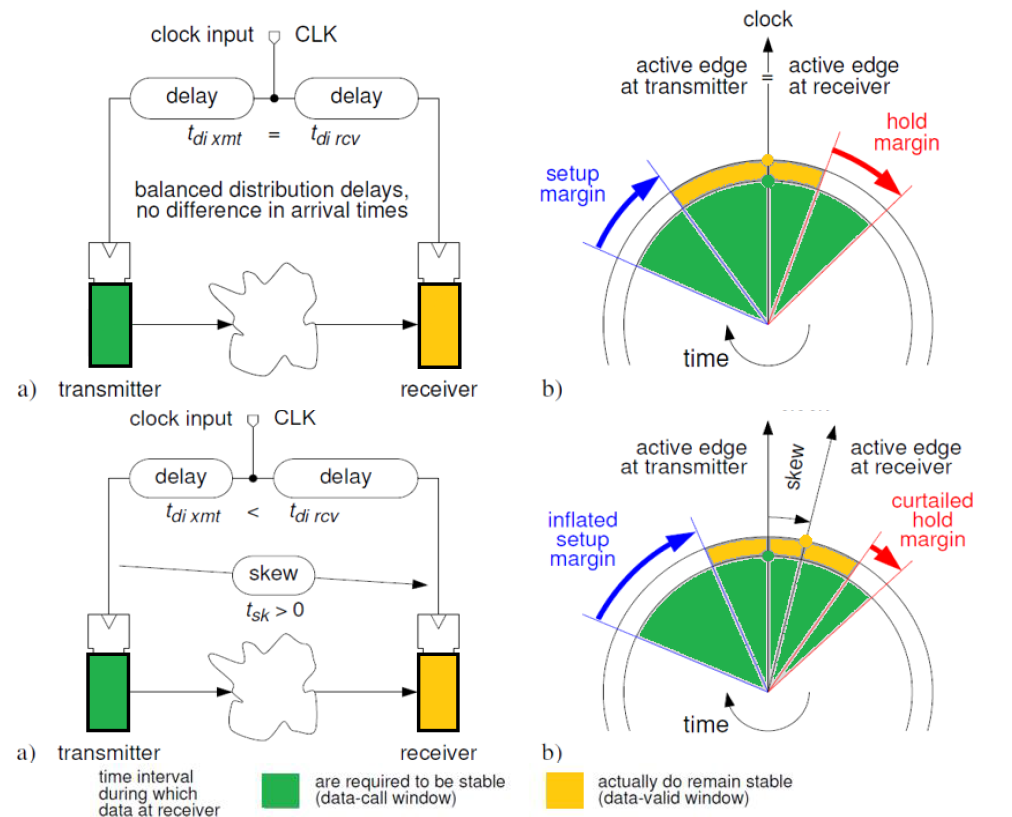
\includegraphics[width=\columnwidth]{Images/slack}
\end{center}

\subsection{Clock}
Alle Clocks sind immer in Nanosek. zu definieren.

\textbf{Beispiel}:
\begin{center}
	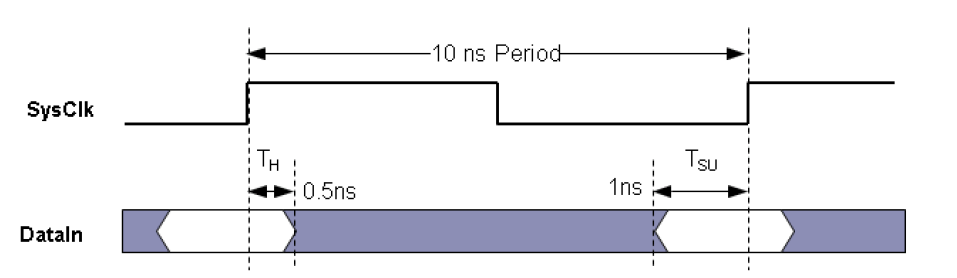
\includegraphics[width=\columnwidth]{Images/clock}
\end{center}

\begin{lstlisting}
-- Clock 100MHz mit 50% Duty Cycle
create_clock -name SysClock -period 10 -waveform {0.000 5.000} [get_ports clk]
set_output_delay -clock SysClock -max 1  [get_ports Dout]
set_output_delay -clock SysClock -min -0.5  [get_ports Dout]
-- latency for external devices
set_clock_latency -source 14 [get_clocks SysClock]
-- jitter definition
set_input_jitter SysClock 0.3
\end{lstlisting}

\subsection{External Components}
\begin{align*}
	t_{input\_delay} &= t_{c\_ext} + t_{pcq\_FF1} + t_{d\_board1} - t_{c\_b1} \\
	t_{output\_delay} &= t_{pcbq\_FF3} + t_{d\_out}
\end{align*}
	
\begin{center}
	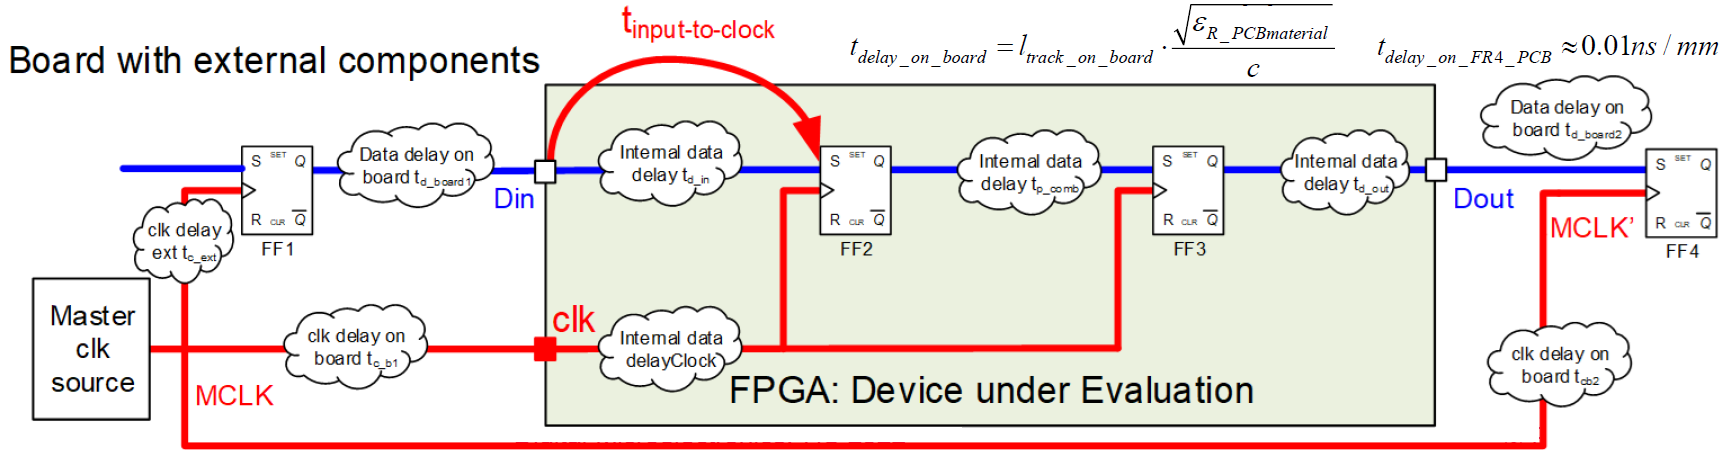
\includegraphics[width=\columnwidth]{Images/clock1}
\end{center}

\section{VHDL}
\subsection{Funktionen}
Funktionen haben mehrere Eingänge und einen Ausgang. Es können dadruch zB Operatoren überschrieben werden.
\begin{itemize}
\item Funktionen können rekursiv aufgerufen werden.
\item Funktionen verwenden keine Signalzuweisungen, sondern nur Variablenzuweisung
\item Der Funktionskörper darf keine Warteanweisung oder eine Signalzuweisung enthalten.
\end{itemize}

\begin{lstlisting}
function PARGEN(AVECT : std_ulogic_vector) return std_ulogic is
	variable PO_VAR : std_ulogic;
begin
	PO_VAR := '1';
	return PO_VAR;
end function PARGEN;
\end{lstlisting}

\subsection{Prozeduren}
Prozeduren haben mehrere Ein und Ausgänge. Sie werden häufig für Test-Banches benutzt und sollten nur Vorsichtig für Hardware code verwendet werden.

Beispiel mit 3 Eingängen und 2 Ausgängen:
\begin{lstlisting}
procedure Comp_3(In1,R :in real; Step :in integer; W1,W2 :out real) is
	variable counter: Integer;
begin
	W1 := 1.43 * In1;
	W2 := 1.0;
	L1: for counter in 1 to Step loop
		W2 := W2 * W1;
		exit L1 when W2 > R;
	end loop L1;
	assert (W2 < R)report "Out of range" severity Error;
end procedure Comp_3;
\end{lstlisting}

\section{Fixed Point}
Unsigned Interger Zahlen $z$ können mit $z=\sum_{k=0}^{n-1}a_k\cdot B^k$ berechnet werden. Signed Interger Zahlen mit $z=-(2^{n-1})\cdot a_{n-1}+\sum_{k=0}^{n-2}a_k\cdot B^k$, wobei $a_k$ die jeweilige Stelle der Bit Zahl entspricht. Um nun Fixed Points zu berechnen, wird das Q-Format verwendet. Dabei steht s/u für singed/unsigend und Qn.m für n=Integer bzw. m=fractional.

\textbf{Beispiel} $10110100$ entspricht im Format uQ2.6:
\[
1\cdot 2^1 + 0\cdot2^0 + 1\cdot2^{-1}+ 1\cdot2^{-2}+ 0\cdot2^{-3}+ 1\cdot2^{-4} = 2.8125
\]
und im Format sQ2.6:
\[
-1\cdot 2^1 + 0\cdot2^0 + 1\cdot2^{-1}+ 1\cdot2^{-2}+ 0\cdot2^{-3}+ 1\cdot2^{-4} = -1.1875
\]

Für die Implementierung in VHDL stehen dazu entweder das Package von IEEE oder die internen Tools zu verfügung. Bei IEEE muss beachtet werden, dass diese nicht immer die Ressourcen optimal ausnutzen und nur teilweise von den synthese Tools unterstützt werden.

\begin{lstlisting}
-- Required libraries for "numeric_std" implementation
library ieee;
use ieee.numeric_std.all;
use ieee.math_real.all;

-- 2.5248 -> binary 10.10000110010110010101
constant REAL_NUM : real := 2.5248;
-- unsigned Q2.6 = 10.100001 = 2.5156 (truncated)
-- decimal point has to be shifted to the right by 6 positions
signal uNumber : unsigned(7 downto 0) := to_unsigned(integer(2.0**6 * REAL_NUM), 8); -- 10100001 --161.5872
-- -2.5248 -> binary 101.0111100110101
constant REAL_NUM : real := -2.5248;
-- signed Q3.5 = 101.01111 = -2.5313 (truncated)
-- the decimal point has to be shifted to the right by 5 positions
signal sNumber : signed(7 downto 0) := to_signed(integer(2.0**5 * REAL_NUM), 8);
\end{lstlisting}

\textbf{Beispiel} Multiplikation
\begin{lstlisting}
constant S_MULTIPLICAND : real := 1.25; -- binary 01.01
constant S_MULTIPLIER : real := -1.25; -- binary 10.11
signal sMultiplicand : signed(3 downto 0) := to_signed(integer(2.0**2 * S_MULTIPLICAND), 4); -- sQ2.2
signal sMultiplier : signed(3 downto 0) := to_signed(integer(2.0**2 * S_MULTIPLIER), 4); -- sQ2.2
signal sProduct : signed(7 downto 0); -- sQ4.4; sQ(n1+n2).(m1+m2)
sProduct <= sMultiplicand * sMultiplier; -- Keep in mind: -- 2 sign bits
-- With one sign bit omitted: -- sQ(n1+n2 - 1).(m1+m2)
signal sProductShort : signed(6 downto 0); -- sQ4.4; sQ(n1+n2 -1).(m1+m2)
sProductShort <= sProduct(6 downto 0);
\end{lstlisting}


Für die IEEE fixed\_pkg sind folgende Zeilen notwendig
\begin{lstlisting}
-- Required libraries for "fixed_pkg" implementation in VHDL 2008
Library ieee;
use ieee.fixed_pkg.all;
use ieee.fixed_float_types.all;

uQ4.6 => ufixed(3 downto -6);
sQ4.6 => sfixed(3 downto -6);

-- example
signal fract : ufixed(-2 downto -3); -- "11" represents 0.011 = 0.375

-- upper and lower index using integer numbers
uNumber <= to_ufixed(5.25, 3, -6); -- ufixed(3 downto -6) = "xxxx,xxxxxx"
-- upper and lower index using the 'high and 'low operator
sNumber <= to_sfixed(-5.25, sNumber'high, sNumber'low);

-- use different round styles
b <= to_ufixed(arg => 2.5248,
  left_index => rounded'HIGH,
  right_index => rounded'LOW,
  overflow_style => FIXED_SATURATE,
  round_style => FIXED_ROUND)
\end{lstlisting}

\begin{center}
	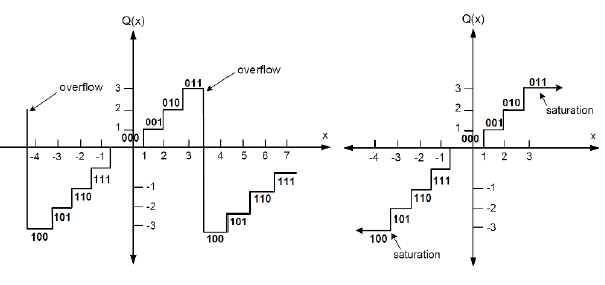
\includegraphics[width=\columnwidth]{Images/saturation}
\end{center}

\textbf{Beispiel} Multiplikation
\begin{lstlisting}
-- fixed_pkg
signal sMultiplicand : sfixed(1 downto -2) := to_sfixed(S_MULTIPLICAND, 1, -2); -- sQ2.2
signal sMultiplier : sfixed(1 downto -2) := to_sfixed (S_MULTIPLIER, 1, -2); -- sQ2.2
signal sProduct : sfixed(3 downto -4); -- Q4.4 -> Q(n1+n2).(m1+m2)

-- sProduct has two sign bits
sProduct <= sMultiplicand * sMultiplier;
-- If second sign bit shall be removed: Q3.4 -> Q(n1+n2-1).(m1+m2)
signal sProductShort : sfixed(2 downto -4);
-- sProductShort has only one sign bit
sProductShort <= resize(sProduct,2,-4);
\end{lstlisting}

\subsubsection{Limits}
\begin{center}
	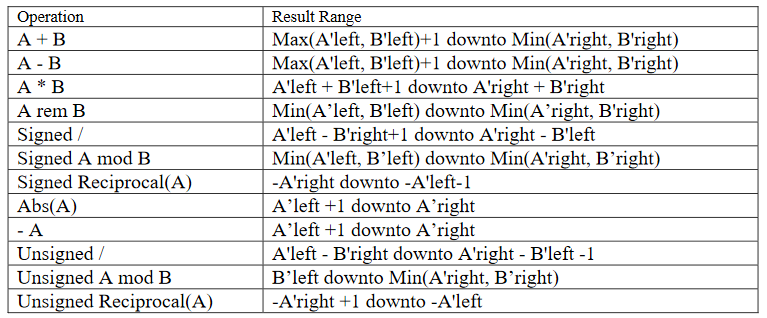
\includegraphics[width=\columnwidth]{Images/limits}
\end{center}

Addition:
\[
Q(n1,m1) + Q(n2,m2) = Q(\max(n1, n2) + 1, \max(m1, m2))
\]
Multiplikation
\[
Q(n1,m1) \cdot Q(n2,m2) = Q(n1 + n2, m1 + m2)
\]
Für signed * signed: MSB ist redundant
\[
Q(n1,m1) \cdot Q(n2,m2) = Q(n1 + n2 -1, m1 + m2+1)
\]
\section{Memory}
Die Grösse wird wie folgt vom Speicher beschrieben:
\begin{center}
	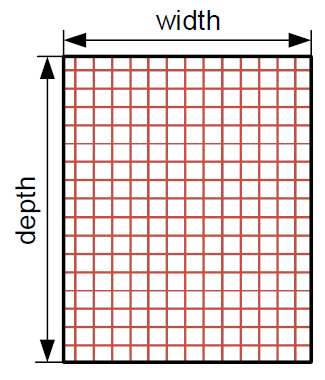
\includegraphics[width=0.7\columnwidth]{Images/memory}
\end{center}
Dabei ist Width die Anzahl an Bits pro Wort und Depth die Anzahl möglichen Addressen $Depth=2^{Address\_width}$. 

Die Schnittstelle ist SinglePort RAM, welches erlaubt ein Zugriff pro Zyklus. True DualPort, wobei damit zwei unterschieliche Addressen im gleichen Zyklus gelesen und beschrieben werden können und Simple DualPort, wo ein Port fürs lesen und der andere fürs schreiben zuständig ist.

\begin{center}
	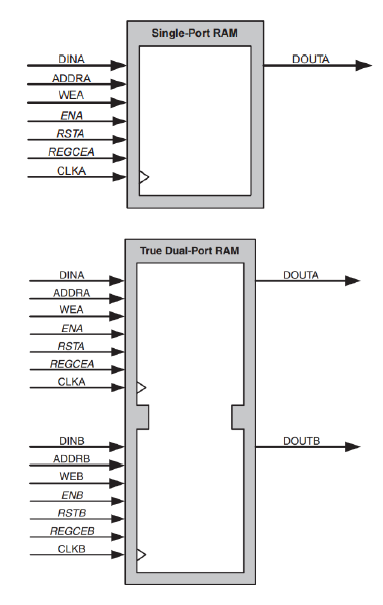
\includegraphics[width=0.7\columnwidth]{Images/ram_interface}
\end{center}
Beispiel für Single-Port RAM interface:
\begin{lstlisting}
library ieee;
use ieee.std_logic_1164.all;
use ieee.numeric_std.all;

entity RAM is
generic(
  ADDR_WIDTH : integer := 8;
  DATA_WIDTH : integer := 8);
port(
  clk : in std_logic;
  addr:in std_logic_vector(ADDR_WIDTH - 1 downto 0);
  din :in std_logic_vector(DATA_WIDTH - 1 downto 0);
  dout:out std_logic_vector(DATA_WIDTH - 1downto 0);
  we, en: in std_logic ); 
end entity RAM;

\end{lstlisting}

\subsection{Distributed RAM}
Werte werden in LUTs gespeichert, schreibt synchron und liest asynchron. Dabei können grosse Speicher instaziiert werden, sind aber nur für kleine schnell erreichbar.
\begin{lstlisting}
architecture RTL of RAM is
  constant MEM_DEPTH : integer := 2 ** ADDR_width;
  type ram_type is array (0 to MEM_DEPTH - 1) of std_logic_vector(DATA_width - 1 downto 0);
  signal dist_ram : ram_type;
  
  attribute ram_style : string;
  attribute ram_style of dist_ram: signal is "distributed";
begin -- distributed RAM with asynchronous read
  DistRAM_write : process(clk)
    begin
      if rising_edge(clk) then
        if en = '1' and we = '1' then
	      dist_ram(to_integer(unsigned(addr))) <= din;
	    end if;
	  end if;
	end process DistRAM_write;
	
	AsyncDistRAM_read: dout <= dist_ram(to_integer(unsigned(addr)));
end RTL;
\end{lstlisting}

\subsection{Block RAM}
Werte werden in Block RAMs à 36kb abgespeichert. Schreiben und lesen ist synchron und ist optimiert für Platz und auch schnell für grössere Strukturen.

\begin{lstlisting}
architecture behavioral of RAM is
  constant MEM_DEPTH : integer := 2 ** ADDR_WIDTH;
  type ram_type is array (0 to MEM_DEPTH - 1) of std_logic_vector(DATA_WIDTH - 1 downto 0);
  signal bram : ram_type;

  attribute ram_style : string;
  attribute ram_style of bram: signal is "block";
begin
  sync_BRAM : process(clk)
    begin
      if rising_edge(clk) then
        if en = '1' then -- if RAM is enabled
          if we = '1' then -- if write is enabled
            bram(to_integer(unsigned(addr))) <= din; -- store din in RAM cell
            dout_block <= din; -- read value back
          else -- synchronous read
            dout_block <= bram(to_integer(unsigned(addr)));
          end if;
        end if;
      end if;
    end process sync_BRAM;
end behavioral;
\end{lstlisting}

\subsection{Dual Port RAM}
Shared Variablen halten Werte auch ausserhalb des Prozesses.
\begin{lstlisting}
architecture behavioral of RAM is
  type mem_type is array (0 to (2 **ADDR) - 1) of std_logic_vector(DATA - 1 downto 0);
  shared variable mem : mem_type;
	
begin
  -- Port A
  process(a_clk) 
  begin
    if rising_edge(a_clk) then
      if a_wr = '1' then
        mem(to_integer(unsigned(a_addr))) := a_din;
      end if;
      a_dout <= mem(to_integer(unsigned(a_addr)));
    end if;
  end process;

  -- Port B
  process(b_clk) 
  begin
    if rising_edge(b_clk) then
      if b_wr = '1' then
        mem(to_integer(unsigned(b_addr))) := b_din;
      end if;
      b_dout <= mem(to_integer(unsigned(b_addr)));
    end if;
  end process;
end behavioral;
\end{lstlisting}

\section{Component Life Cycle}
\begin{itemize}
	\item A \textbf{Pre-Production} IP core is in general public release for a device family, but has not completed qualification for use in production designs.*
	\item A \textbf{Production} IP core is one which is provi-ded for general public release, and has been verified using production speed files.
	\item A \textbf{Discontinued }IP core is one that Xilinx has decided to discontinue
	\item A \textbf{Superseded} IP core is one that has been replaced by a newer version.
	\item A core in the \textbf{Removed} state no longer ships in Vivado releases.
\end{itemize}

\subsection{Versioning}
major\#.minor\#.Rev\# numbering scheme
\begin{center}
	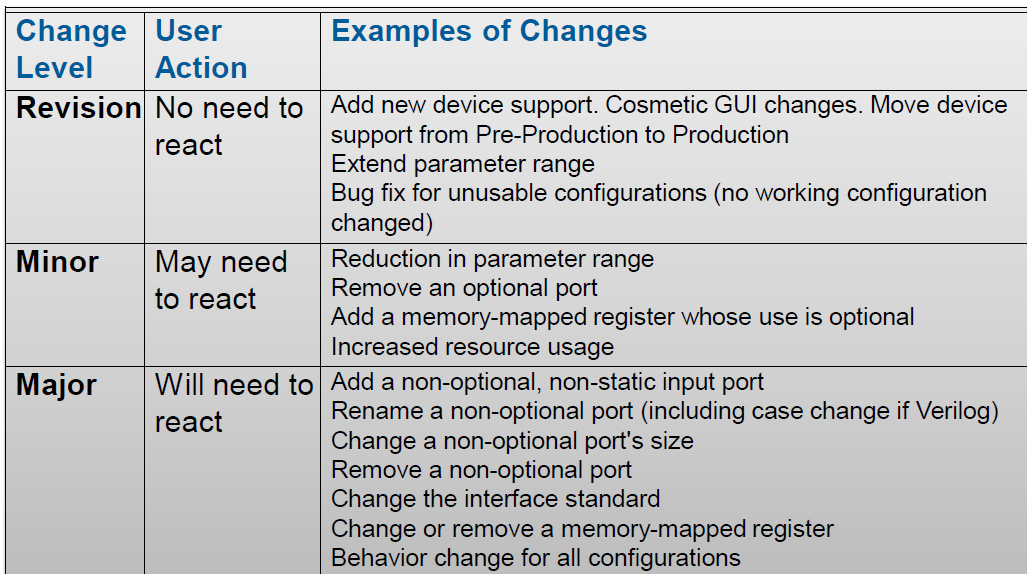
\includegraphics[width=\columnwidth]{Images/versioning}
\end{center}

\section{Serial Interfaces}
\subsection{SPI}
Benötigt 3 + \#Slaves Pins und wird max bis 100MHz betrieben. Eine Transaktion starte, wenn CS auf 0 springt.
\begin{center}
	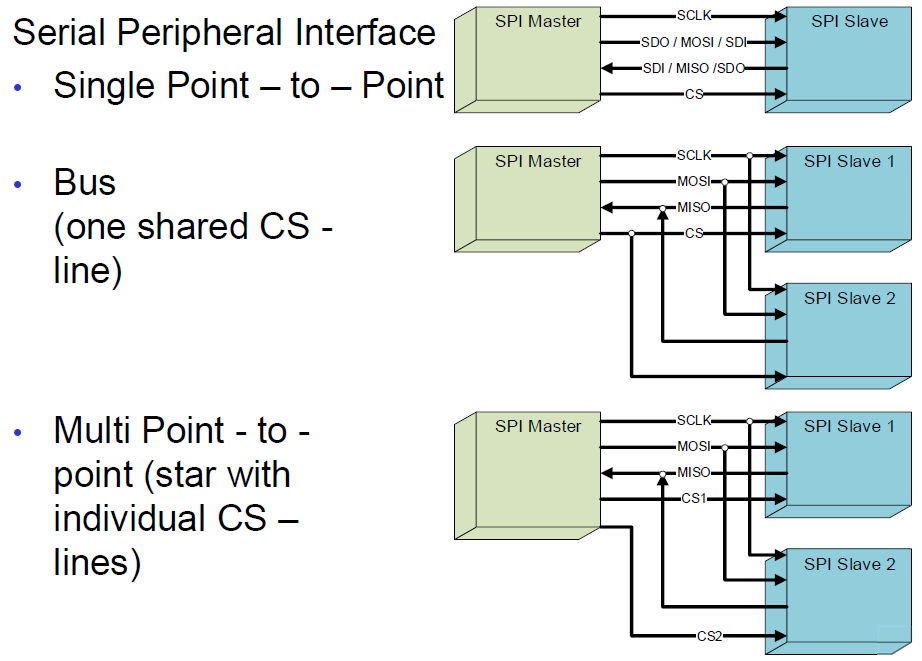
\includegraphics[width=\columnwidth]{Images/spi}
\end{center}
\begin{center}
	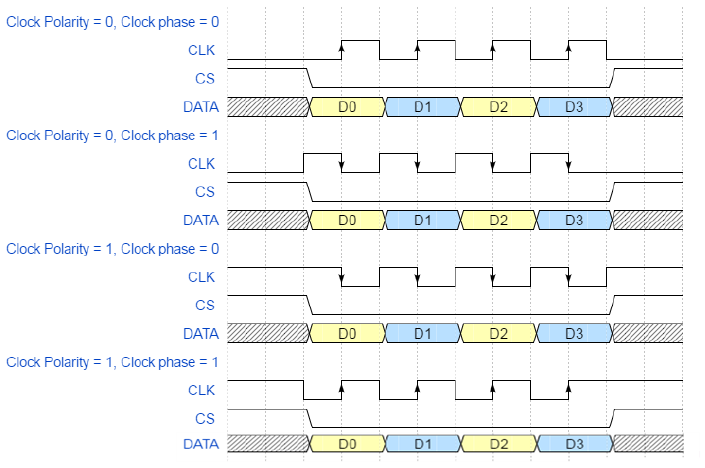
\includegraphics[width=\columnwidth]{Images/spi_mode}
\end{center}

\subsection{I$^2$C}
Benötigt zwei \textbf{bidirectionale} Leitungen, unabhängig von Anzahl Slaves und wird zwischen 100kbit/s bis 3.4Mbit/s betrieben. Wichtig dabei, beide Leitungen müssen immer einen Pull-Up Widerstand haben.
\begin{center}
	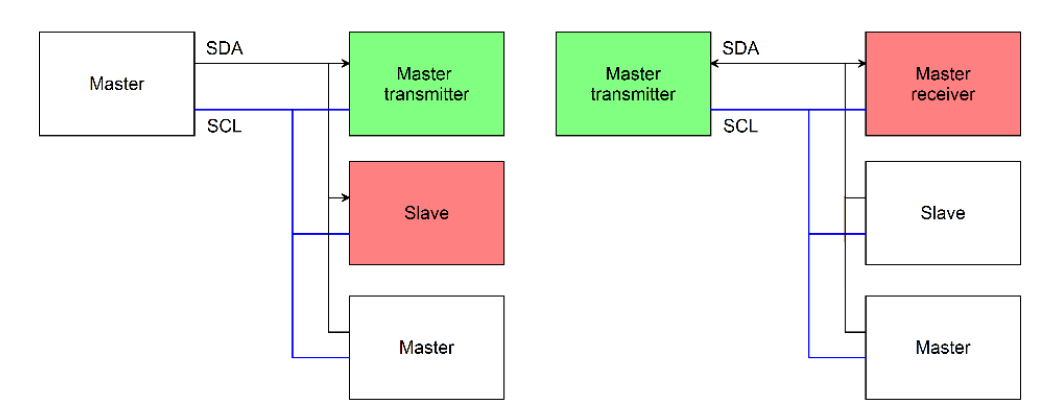
\includegraphics[width=0.7\columnwidth]{Images/i2c}
\end{center}
\begin{center}
	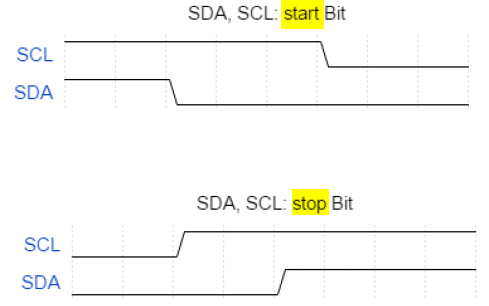
\includegraphics[width=0.7\columnwidth]{Images/i2c_start}
\end{center}

Timing Übersicht:
\begin{center}
	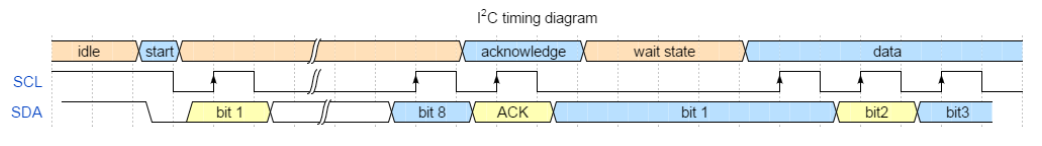
\includegraphics[width=\columnwidth]{Images/i2c_timing}
\end{center}

\section{Parallel Interface}
\subsection{AXI}
AXI ist ein 1-to-1 Interface (Master-Slave) mit fünf unabhängigen Channels:
\begin{center}
	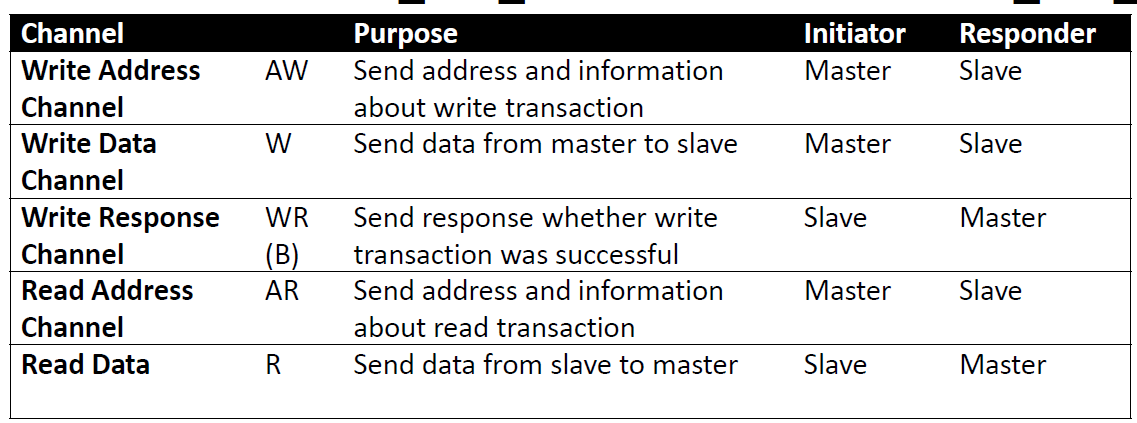
\includegraphics[width=\columnwidth]{Images/axi}
\end{center}

Dabei gibt es drei Unterschiedliche Varianten:
\begin{itemize}
	\item \textbf{AXI4}(-Full), unterstützt BurstMode bis zu 256 Daten Packeten pro Address und ist Memmory Mapped
	\item \textbf{AXI4-Lite}, Keine Burst und ist Memory Mapped für einzelne Transaktionen
	\item \textbf{AXI4-Stream}, Für Streaming Anwendungen und daher nur Schreib-Channel. Nur Daten von Master zu Slave möglich mit unlimitierten Burst grösse.
\end{itemize}

\subsubsection{Interconnect}
Da AXI eine Schnittstelle zwischen Master-Slave ist, wird ein Interconnect für die n-m Kommuikation benötig. Dieser Interconnect entscheided auf basis der Address, zu welchem Slave er die Packete routen muss.
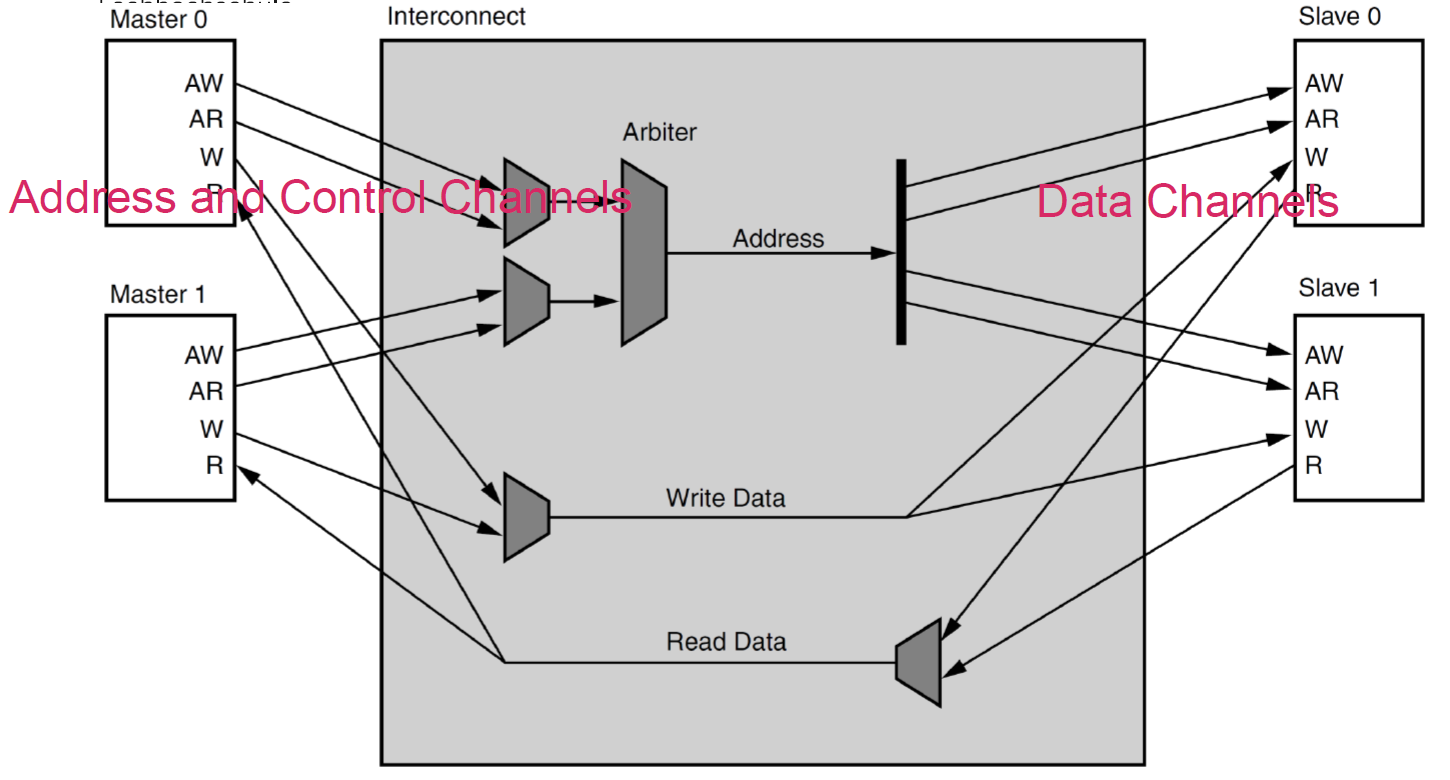
\includegraphics[width=\columnwidth]{Images/interconnect}


\end{document}